%!TEX root = ../../thesis.tex

\chapter{Methodology}
\label{methodology}

This chapter presents the design and implementation of FlatCityBuf, a cloud-optimised binary format for 3D city models based on CityJSONSeq. The proposed approach addresses the limitations of existing formats through efficient binary encoding, spatial indexing, attribute indexing, and support for partial data retrieval.

\section{Overview}
\label{methodology:overview}

\subsection{Methodology Approach}
\label{methodology:overview:approach}

Current 3D city model formats like CityGML, CityJSON, and \ac{cjseq} exhibit limitations in cloud environments with large-scale datasets, including retrieval latency, inefficient spatial querying without additional software support, and insufficient support for partial data access.

This chapter addresses these limitations through three interconnected objectives:

\begin{enumerate}
  \item Development of a binary encoding strategy using FlatBuffers that preserves semantic richness while achieving faster read performance
  \item Implementation of dual indexing mechanisms—spatial (packed Hilbert R-tree) and attribute-based (\ac{s+tree}) that accelerate query performance
  \item Integration of cloud-native data access patterns through \ac{http} Range Requests, enabling partial data retrieval
\end{enumerate}

\subsection{Outcomes of the Methodology}
\label{methodology:overview:outcomes}

Before delving into the methodological details, it is important to highlight the tangible research outcomes produced through this work:

\begin{itemize}
  \item \textbf{Data format specification}: FlatCityBuf, a cloud-optimised binary format for 3D city models that maintains semantic compatibility with CityJSON while enabling efficient cloud-based access patterns.

  \item \textbf{Reference implementation}: A comprehensive Rust library for encoding, decoding, and querying FlatCityBuf files, accompanied by command-line interface (CLI) tools for conversion and validation.

  \item \textbf{Web demonstration}: A web-based prototype application that showcases the partial data retrieval capabilities of FlatCityBuf through \ac{http} range requests, demonstrating practical performance improvements in real-world scenarios.

  \item \textbf{Performance evaluation}: A comprehensive performance evaluation of the proposed methodology, demonstrating the benefits of the proposed approach in terms of file size, query latency, memory usage, and other relevant metrics.
\end{itemize}

These outcomes collectively address the research objectives by providing both a theoretical framework and practical implementations that validate the approach to cloud-optimised 3D city model storage and retrieval.

\subsection{File Structure Overview}
\label{methodology:overview:file_structure}

The FlatCityBuf format implements a structured binary encoding with five sequentially arranged components:

\begin{itemize}
  \item \textbf{Magic bytes}: Eight-byte identifier ('F', 'C', 'B', '0', '1', '0', '0', '0') for format validation
  \item \textbf{Header section}: Contains metadata, attributes schema definitions, and CityJSON properties
  \item \textbf{Spatial index}: Implements a Packed Hilbert R-tree \citep{Kamel_Faloutsos_1993} for efficient geospatial queries
  \item \textbf{Attribute index}: Utilises a \ac{s+tree} for accelerated attribute-based filtering
  \item \textbf{Features section}: Stores features encoded as FlatBuffers tables
\end{itemize}

\begin{figure}[h]
  \centering
  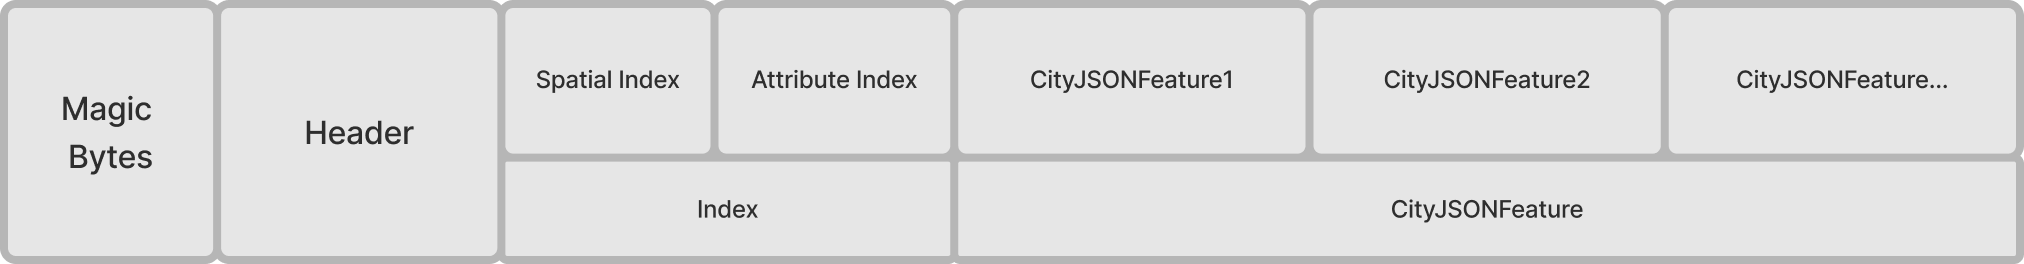
\includegraphics[width=0.8\textwidth]{figs/methodology/file_structure.png}
  \caption{Physical layout of the FlatCityBuf file format, showing section boundaries and alignment considerations for optimised range requests}
  \label{fig:methodology:file-structure}
\end{figure}

This sequence-based structure enables incremental file access through \ac{http} Range Requests—critical for cloud-based applications where minimising data transfer is essential.

\subsection{Note on Binary Encoding}
\label{methodology:overview:note_on_binary_encoding}
FlatCityBuf follows two key conventions for encoding binary data throughout the file format:

\begin{enumerate}
  \item \textbf{Size-prefixed FlatBuffers}: All FlatBuffers records (header and features) include a 4-byte unsigned integer prefix indicating the buffer size. This enables programs to know the size of the record without parsing the entire content. The FlatBuffers \ac{api} implements this through \texttt{finish\_size\_prefixed} or equivalent language-specific methods.
  \item \textbf{Little-endian encoding}: For data encoded outside FlatBuffers records (particularly in spatial and attribute indices), little-endian byte ordering is consistently applied, matching the endianness convention used within FlatBuffers records. This includes numeric values such as 32-bit and 64-bit integers, floating-point numbers, and offset values within indices.
\end{enumerate}

These conventions ensure consistency across the file format and maximise compatibility with modern \ac{cpu} architectures, most of which use little-endian byte ordering. The size-prefixing mechanism is particularly important for cloud-based access patterns, as it facilitates precise \ac{http} Range Requests when retrieving specific file segments.
